% This is samplepaper.tex, a sample chapter demonstrating the
% LLNCS macro package for Springer Computer Science proceedings;
% Version 2.21 of 2022/01/12
%
\documentclass[runningheads]{llncs}
%
\usepackage[T1]{fontenc}
% T1 fonts will be used to generate the final print and online PDFs,
% so please use T1 fonts in your manuscript whenever possible.
% Other font encondings may result in incorrect characters.
%
\usepackage{graphicx}
% Used for displaying a sample figure. If possible, figure files should
% be included in EPS format.
%
% If you use the hyperref package, please uncomment the following two lines
% to display URLs in blue roman font according to Springer's eBook style:
%\usepackage{color}
%\renewcommand\UrlFont{\color{blue}\rmfamily}
%
\usepackage{amsmath}
\usepackage{csquotes}
\usepackage{listings}
\usepackage{diagbox}
\usepackage{tikz}

\usetikzlibrary{shapes.geometric, arrows}
\tikzstyle{startstop} = [rectangle, rounded corners, minimum width=2cm, minimum height=0.7cm,text centered, draw=black, fill=red!30]
\tikzstyle{io} = [trapezium, trapezium left angle=70, trapezium right angle=110, minimum width=2cm, minimum height=0.7cm, text centered, draw=black, fill=blue!30]
\tikzstyle{process} = [rectangle, minimum width=2cm, minimum height=0.7cm, text centered, draw=black, fill=orange!30]
\tikzstyle{decision} = [diamond, minimum width=2cm, minimum height=0.7cm, text centered, draw=black, fill=green!30]
\tikzstyle{arrow} = [thick,->,>=stealth]

\lstdefinelanguage{Clojure}
{morekeywords={*,*1,*2,*3,*agent*,*allow-unresolved-vars*,*assert*,*clojure-version*,*command-line-args*,
*compile-files*,*compile-path*,*e,*err*,*file*,*flush-on-newline*,*in*,*macro-meta*,
*math-context*,*ns*,*out*,*print-dup*,*print-length*,*print-level*,*print-meta*,*print-readably*,
*read-eval*,*source-path*,*use-context-classloader*,*warn-on-reflection*,+,-,->,->>,..,/,:else,
<,<=,=,==,>,>=,@,accessor,aclone,add-classpath,add-watch,agent,agent-errors,aget,alength,alias,
all-ns,alter,alter-meta!,alter-var-root,amap,ancestors,and,apply,areduce,array-map,aset,
aset-boolean,aset-byte,aset-char,aset-double,aset-float,aset-int,aset-long,aset-short,assert,
assoc,assoc!,assoc-in,associative?,atom,await,await-for,await1,bases,bean,bigdec,bigint,binding,
bit-and,bit-and-not,bit-clear,bit-flip,bit-not,bit-or,bit-set,bit-shift-left,bit-shift-right,
bit-test,bit-xor,boolean,boolean-array,booleans,bound-fn,bound-fn*,butlast,byte,byte-array,
bytes,cast,char,char-array,char-escape-string,char-name-string,char?,chars,chunk,chunk-append,
chunk-buffer,chunk-cons,chunk-first,chunk-next,chunk-rest,chunked-seq?,class,class?,
clear-agent-errors,clojure-version,coll?,comment,commute,comp,comparator,compare,compare-and-set!,
compile,complement,concat,cond,condp,conj,conj!,cons,constantly,construct-proxy,contains?,count,
counted?,create-ns,create-struct,cycle,dec,decimal?,declare,def,definline,defmacro,defmethod,
defmulti,defn,defn-,defonce,defprotocol,defstruct,deftype,delay,delay?,deliver,deref,derive,
descendants,destructure,disj,disj!,dissoc,dissoc!,distinct,distinct?,do,do-template,doall,doc,
dorun,doseq,dosync,dotimes,doto,double,double-array,doubles,drop,drop-last,drop-while,empty,empty?,
ensure,enumeration-seq,eval,even?,every?,false,false?,ffirst,file-seq,filter,finally,find,find-doc,
find-ns,find-var,first,float,float-array,float?,floats,flush,fn,fn?,fnext,for,force,format,future,%
future-call,future-cancel,future-cancelled?,future-done?,future?,gen-class,gen-interface,gensym,
get,get-in,get-method,get-proxy-class,get-thread-bindings,get-validator,hash,hash-map,hash-set,
identical?,identity,if,if-let,if-not,ifn?,import,in-ns,inc,init-proxy,instance?,int,int-array,
integer?,interleave,intern,interpose,into,into-array,ints,io!,isa?,iterate,iterator-seq,juxt,
key,keys,keyword,keyword?,last,lazy-cat,lazy-seq,let,letfn,line-seq,list,list*,list?,load,load-file,
load-reader,load-string,loaded-libs,locking,long,long-array,longs,loop,macroexpand,macroexpand-1,
make-array,make-hierarchy,map,map?,mapcat,max,max-key,memfn,memoize,merge,merge-with,meta,
method-sig,methods,min,min-key,mod,monitor-enter,monitor-exit,name,namespace,neg?,new,newline,
next,nfirst,nil,nil?,nnext,not,not-any?,not-empty,not-every?,not=,ns,ns-aliases,ns-imports,
ns-interns,ns-map,ns-name,ns-publics,ns-refers,ns-resolve,ns-unalias,ns-unmap,nth,nthnext,num,
number?,odd?,or,parents,partial,partition,pcalls,peek,persistent!,pmap,pop,pop!,pop-thread-bindings,
pos?,pr,pr-str,prefer-method,prefers,primitives-classnames,print,print-ctor,print-doc,print-dup,
print-method,print-namespace-doc,print-simple,print-special-doc,print-str,printf,println,println-str,
prn,prn-str,promise,proxy,proxy-call-with-super,proxy-mappings,proxy-name,proxy-super,
push-thread-bindings,pvalues,quot,rand,rand-int,range,ratio?,rational?,rationalize,re-find,
re-groups,re-matcher,re-matches,re-pattern,re-seq,read,read-line,read-string,recur,reduce,ref,
ref-history-count,ref-max-history,ref-min-history,ref-set,refer,refer-clojure,reify,
release-pending-sends,rem,remove,remove-method,remove-ns,remove-watch,repeat,repeatedly,
replace,replicate,require,reset!,reset-meta!,resolve,rest,resultset-seq,reverse,reversible?,
rseq,rsubseq,second,select-keys,send,send-off,seq,seq?,seque,sequence,sequential?,set,set!,
set-validator!,set?,short,short-array,shorts,shutdown-agents,slurp,some,sort,sort-by,sorted-map,
sorted-map-by,sorted-set,sorted-set-by,sorted?,special-form-anchor,special-symbol?,split-at,
split-with,str,stream?,string?,struct,struct-map,subs,subseq,subvec,supers,swap!,symbol,symbol?,
sync,syntax-symbol-anchor,take,take-last,take-nth,take-while,test,the-ns,throw,time,to-array,
to-array-2d,trampoline,transient,tree-seq,true,true?,try,type,unchecked-add,unchecked-dec,
unchecked-divide,unchecked-inc,unchecked-multiply,unchecked-negate,unchecked-remainder,
unchecked-subtract,underive,unquote,unquote-splicing,update-in,update-proxy,use,val,vals,
var,var-get,var-set,var?,vary-meta,vec,vector,vector?,when,when-first,when-let,when-not,
while,with-bindings,with-bindings*,with-in-str,with-loading-context,with-local-vars,
with-meta,with-open,with-out-str,with-precision,xml-seq,zero?,zipmap
},
   sensitive,
   alsodigit=-,
   morecomment=[l];,
   morestring=[b]"
  }[keywords,comments,strings]

\begin{document}
\lstset{language=Clojure}
%
\title{Comparing Regular Grammars and Regular Expressions created by Genetic Programming}
%
\titlerunning{Regular Grammars and Regular Expressions via GP}
% If the paper title is too long for the running head, you can set
% an abbreviated paper title here
%
\author{Markus Fruhmann\inst{1}\orcidID{11844261}}
%
\authorrunning{M. Fruhmann}
% First names are abbreviated in the running head.
% If there are more than two authors, 'et al.' is used.
%
\institute{Institute of Softwaretechnology, Technical University of Graz}
%
\maketitle              % typeset the header of the contribution
%
\begin{abstract}
The abstract should briefly summarize the contents of the paper in
150--250 words.

\keywords{First keyword  \and Second keyword \and Another keyword.}
\end{abstract}
%
%
%
\section{Introduction}
TODO

\section{Related Work}
The representation of languages with more general rules or structures is not new. Achievements in this field have already been made by Alberto Bartoli et al, who published papers on the creation of regular grammars with genetic programming and by the research team of Bernhard K. Aichernig, who created AALpy, a python library that uses active automata learning algorithms to represent languages as finite-state machines.

An interesting application Alberto Bartoli discovered for genetic programming is regex golf, where the shortest expression should be created for a given list of valid and invalid words. He and his team were able to construct a genetic programming system, that generates solutions which are highly competitive with respect to human players and can be created in a similar time-frame as well \cite{regolf-2014}.

The goal of AALpy is to use automata learning for model-based verification by learning the behaviours of unknown systems and modeling it as a finite-state machine \cite{aalpy-2022}.

\section{Preliminaries}
This section will lay the groundwork for the implementation and experiments. We will first define what languages are and dive into the two representations for languages used in this project, regular expressions and regular grammars. The final part will cover the parts required for genetic programming.

\subsection{Definition of Languages}
Before talking about creating regular expressions or regular grammars for different languages, we first have to define what a language is.

Each language consists of an alphabet, which is a nonempty, finite set of characters. This alphabet will be noted as $\Sigma$.
Using this alphabet, we are able to construct words. A word is simply a string, a finite sequence of characters from the alphabet \cite[17]{fla-2017}.

In our case, all characters of an alphabet are lowercase letters \underline{a}, \underline{b}, \underline{c},... for elements of $\Sigma$, since these letters signify the non-terminals in our regular grammars.
Each word $\omega$ of our language has a length, denoted by $|\omega|$. The length can be obtained by counting all characters that make up a specific word. A very important special word is the empty string $\lambda$, which does not contain any characters and therefore has a length of 0 \cite[17]{fla-2017}.

As we now have defined the alphabet $\Sigma$, a word of the alphabet $\omega$ and the empty string $\lambda$, we can now look at two special alphabets, $\Sigma^{+}$ and $\Sigma^{*}$. $\Sigma^{*}$ contains all words that can be created using the characters in $\Sigma$, including the empty string $\lambda$. To exclude $\lambda$, we can define $\Sigma^{+}$ as follows:
\begin{equation}
\Sigma^{+}=\Sigma^{*} - {\lambda}.
\end{equation}

In contrast to the finite nature of $\Sigma$, $\Sigma^{*}$ and $\Sigma^{+}$ are both infinite, since the length of the strings in these sets is not limited in any way. Therefore, a language $L$ can be defined as a subset of $\Sigma^{*}$, where the corresponding alphabet $\Sigma$ contains all different characters used in $L$. This means, that two languages $L1$ and $L2$ might share the same alphabet $\Sigma$, but each could contain a subset of $\Sigma^{*}$ such that
\begin{equation}
L_{1} \cap L_{2} = \oslash .
\end{equation}

Since languages are just sets by definition, as they are subsets of the set $\Sigma^{*}$, the operations union, intersection and difference are immediately applicable. Concatenating two languages $L1$ and $L2$ will result in every element of $L1$ being concatenated with every element of $L2$. Another important definition is $L^n$, which is the language $L$ concatenated with itself $n$ times. Following special cases
\begin{align}
L^0 = {\lambda}\\
L^1 = L
\end{align}
the star-closure
\begin{equation}
L^* = L^0 \cup L^1 \cup L^2 ...
\end{equation}
and the positive closure
\begin{equation}
L^+ = L^1 \cup L^2 ...
\end{equation}
are applicable to every language $L$ \cite[19-20]{fla-2017}.

With this solid definition of languages, we are able to define regular expressions and regular grammars in the following sections.


\subsection{Regular Expressions}
When describing a language with regular expressions in a formal way, a special notation is used. This notation consists of words created from characters of an alphabet $\Sigma$, parentheses $()$ and the operators $+$, $\cdot$ and $*$. The operators $+$, $\cdot$ and $*$ signify different set operations on a language $L$. $+$ is denotes the union, $\cdot$ denotes concatenation and $*$ denotes the star-closure \cite[74]{fla-2017}.

We can define regular expressions in a formal matter the following way:
\begin{quote}
    Let $\Sigma$ be a given alphabet. Then
    \begin{enumerate}
        \item $\oslash$, $\lambda$, and $a \in \Sigma$ are all regular expressions. These are called *primitive regular expressions*.
        \item If $r_1$ and $r_2$ are regular expressions, so are $r_1 + r_2$, $r_1 \cdot r_2$, $r_1^{\*}$ and $(r_1)$.
        \item A string is a regular expression if and only if it can be derived from the primitive regular expressions by a finite number of applications of the rules in (2) \cite[74]{fla-2017}.
    \end{enumerate}
\end{quote}

The some small problems arise, when many of the operators defined above are used in conjunction. To further elaborate this, let's consider the regular expression $a \cdot b + c$. We now have two valid options to represent this regular expression: $r_1 = a \cdot b$ and $r_2 = c$ which results in the language $L(a \cdot b + c)= {ab,c}$ or $r_1=a$ and $r_2=b+c$ which results in $L(a \cdot b + c)={ab,ac}$. To prevent such ambiguity, we could either parenthesize all expressions, but this would be hard to read. Therefore, a precedence is given to each operator, which ensures that each one is evaluated in the correct order. This means, that $*$ star-closure precedes $\cdot$ concatenation, which precedes $+$ union. Furthermore, the operator for concatenation can be omitted and we can rewrite $r_1 \cdot r_2$ to $r_1 r_2$ \cite[76]{fla-2017}.

With this formal definition of regular grammars and their operators, we can now define the different operators used in modern pattern matchers for regular expressions, as they differ from their formal counterparts. In modern regular expression syntax, the operator for concatenation $\cdot$ is always omitted. The union operator $+$ can be replaced with the logical OR, $|$, since it also creates a set consisting of the elements on each side of $|$ where one of them can be selected to match. The $+$ operator now signifies the positive closure, while the $*$ operator does not change and still signifies the star-closure.


\subsection{Regular Grammars}
Regular grammars are another way to represent languages and language families, that can be represented with an automaton. Two types of regular grammars are possible \cite[92]{fla-2017}.
\begin{quote}
A grammar $G=(V,T,S,P)$ is said to be \textbf{right-linear} if all productions are of the form
\begin{align}
A \rightarrow xB,\\
A \rightarrow x,
\end{align}
where $A,B \in V$, and $x \in T_{\*}$. A grammar is said to be \textbf{left-linear} if all productions are of the form
\begin{equation}
A \rightarrow Bx,
\end{equation}
or
\begin{equation}
A \rightarrow x.
\end{equation}
A \textbf{regular grammar} is one that is either right-linear or left-linear \cite[92]{fla-2017}.
\end{quote}

A defining characteristic of regular grammars is, that at most one variable can appear on the right side of any production rule and the variable must consistently be placed on the far right or the far left on the right side of the production rule \cite[92]{fla-2017}.

In the following sections, the grammars used will strongly adhere to the EBNF notation as it is defined in ISO/IEC 14977 from 1996. This means, that instead of $\rightarrow$, $=$ will be used to define a production rule and all possible options for said rule are separated with $|$. For our purposes, the empty string will be represented by $\epsilon$ instead of $\lambda$, but $\lambda$ will be used in formal definitions. Consider following example:
\begin{align}
A \rightarrow xA,\\
A \rightarrow xB,\\
B \rightarrow yB,\\
B \rightarrow \lambda,
\end{align}
can be rewritten to
\begin{align}
A = xA|xB;\\
B = yb|\epsilon;
\end{align}
which now adheres to the aforementioned EBNF notation. Note, that each rule is separated by a semicolon as well, which further ties into the definition of EBNF.

\subsection{Genetic Programming}
After defining the basis for the representation of languages with regular expressions and regular grammars, we can now move on to the last part needed for this project, \textbf{genetic programming}, which itself is based on \textbf{genetic algorithms}.
\begin{quote}
The \emph{genetic algorithm} is a highly parallel mathematical algorithm that transforms a set (\emph{population}) of individual mathematical objects [\ldots{}], each with an associated \emph{fitness} value, into a new population (i.e., the next \emph{generation} $M$) using operations patterned after the Darwinian principle of reproduction and survival of the fittest and after naturally occurring genetic operations [\ldots{}] \cite[18]{gp1-1993}.
\end{quote}
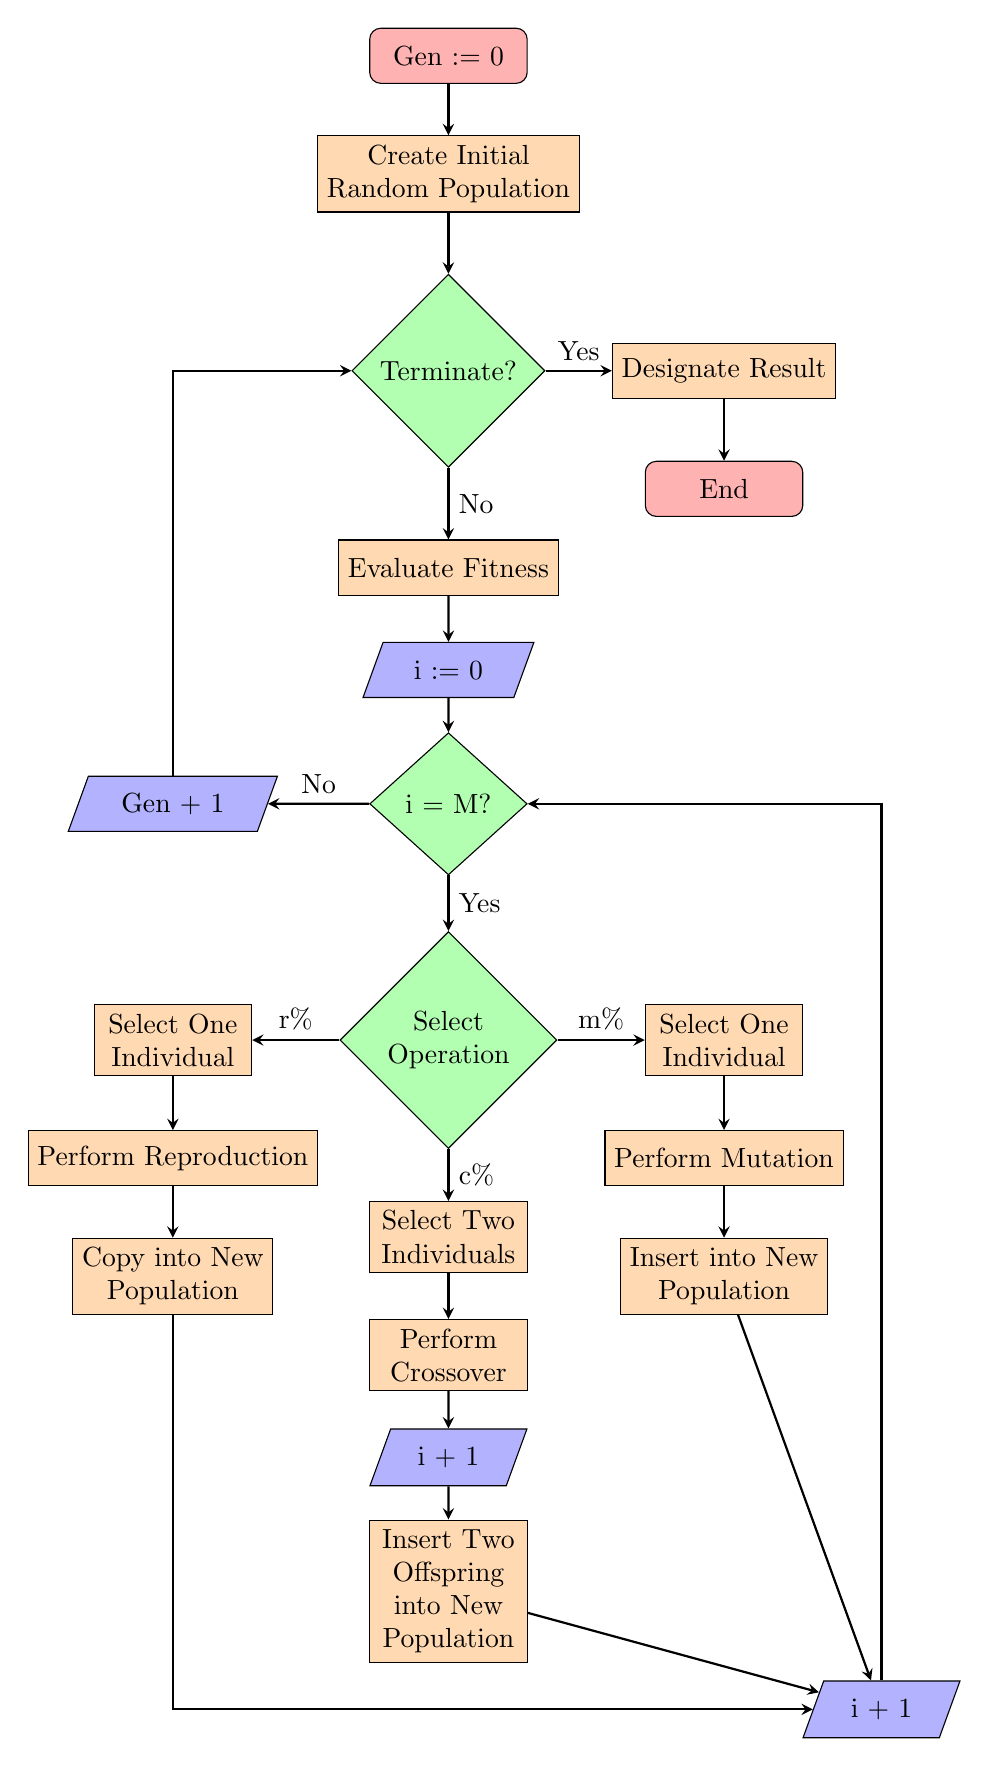
\begin{tikzpicture}[node distance=1.5cm]
% NODES
\node (start) [startstop] {Gen := 0};
\node (create-initial) [process, below of=start, align=center] {Create Initial \\ Random Population};
\node (terminate?) [decision, below of=create-initial, yshift=-1cm] {Terminate?};

\node (result) [process, right of=terminate?, xshift=2cm] {Designate Result};
\node (end) [startstop, below of=result] {End};

\node (fitness) [process, below of=terminate?, yshift=-1cm] {Evaluate Fitness};
\node (new-cnt) [io, below of=fitness, yshift=0.2cm] {i := 0};

\node (breed?) [decision, below of=new-cnt, yshift=-0.2cm] {i = M?};
\node (next-gen) [io, left of=breed?, xshift=-2cm] {Gen + 1};

\node (select) [decision, below of=breed?, align=center, yshift=-1.5cm] {Select \\ Operation};

\node (select-crossover) [process, below of=select, align=center, yshift=-1cm] {Select Two \\ Individuals};
\node (crossover) [process, below of=select-crossover, align=center] {Perform \\ Crossover};
\node (inc-crossover) [io, below of=crossover, yshift=0.2cm] {i + 1};
\node (insert-crossover) [process, below of=inc-crossover, align=center, yshift=-0.2cm] {Insert Two \\ Offspring \\ into New \\ Population};

\node (select-reproduction) [process, left of=select, align=center, xshift=-2cm] {Select One \\ Individual};
\node (reproduction) [process, below of=select-reproduction] {Perform Reproduction};
\node (copy-individual) [process, below of=reproduction, align=center] {Copy into New \\ Population};

\node (select-mutation) [process, right of=select, align=center, xshift=2cm] {Select One \\ Individual};
\node (mutation) [process, below of=select-mutation] {Perform Mutation};
\node (insert-mutation) [process, below of=mutation, align=center] {Insert into New \\ Population};

\node (inc-population) [io, below of=insert-mutation, xshift=2cm, yshift=-4cm] {i + 1};

% ARROWS
\draw [arrow] (start) -- (create-initial);
\draw [arrow] (create-initial) -- (terminate?);

\draw [arrow] (terminate?) -- node[anchor=south] {Yes} (result);
\draw [arrow] (result) -- (end);

\draw [arrow] (terminate?) -- node[anchor=west] {No} (fitness);
\draw [arrow] (fitness) -- (new-cnt);

\draw [arrow] (new-cnt) -- (breed?);
\draw [arrow] (breed?) -- node[anchor=south] {No} (next-gen);
\draw [arrow] (next-gen) |- (terminate?);

\draw [arrow] (breed?) -- node[anchor=west] {Yes} (select);

\draw [arrow] (select) -- node[anchor=west] {c\%} (select-crossover);
\draw [arrow] (select-crossover) -- (crossover);
\draw [arrow] (crossover) -- (inc-crossover);
\draw [arrow] (inc-crossover) -- (insert-crossover);
\draw [arrow] (insert-crossover) -- (inc-population);

\draw [arrow] (select) -- node[anchor=south] {r\%} (select-reproduction);
\draw [arrow] (select-reproduction) -- (reproduction);
\draw [arrow] (reproduction) -- (copy-individual);
\draw [arrow] (copy-individual) |- (inc-population);

\draw [arrow] (select) -- node[anchor=south] {m\%} (select-mutation);
\draw [arrow] (select-mutation) -- (mutation);
\draw [arrow] (mutation) -- (insert-mutation);
\draw [arrow] (insert-mutation) -- (inc-population);

\draw [arrow] (inc-population) |- (breed?);
\end{tikzpicture}\\
\cite[29, Figure 3.1]{gp1-1993}.

\subsubsection{Function and Terminal Set}
In genetic programming, like in every other adaptive system, at least one structure is altered and adapted during learning. What makes genetic programming special, is, that instead of a single point, all individual elements of the search space are being adapted, instead of a single element. This means, that genetic methods can search hundreds or thousands of points in the search space in parallel. The individual structures that are processed by genetic programming are hierarchical computer programs. The set of possible individual structures is given by all possible compositions of elements from a function set \texttt{F} and a terminal set \texttt{T}. Each function of \texttt{F} takes a specified number of arguments, which signifies a functions \emph{arity}. These functions can be arithmetic operations, boolean operators or any other function that is domain-specific. Terminals can either be variable atoms, like the state of a system, or constant values, like the number \texttt{3} or the boolean value \texttt{true} \cite[79-80]{gp1-1993}.

A very important property of each function of \texttt{F} is \emph{closure}. Closure means, that the output of any function in $f_1 \in F$, may possibly be used as input for any other function $f_2 \in F$. This also means, that every function that could produce an error, like $\div$ when dividing by 0, has to handle such cases in a gracious way that produces a reasonable alternative result. In this case, a reasonable output could be 1, when dividing by 0 \cite[81-82]{gp1-1993}.

The other very important property for functions \texttt{F} and terminals \texttt{T} for a given problem is \emph{sufficiency}. Sufficiency means, that the set of all possible individual structures using \texttt{F} and \texttt{T} can yield a solution for the given problem. It is therefore necessary to identify the functions and terminals that have this sufficient power of expression, even if this task might sometimes be impossible and the number of variables has to be restricted to a set that comes close enough to a perfect solution \cite[86-87]{gp1-1993}.

\subsubsection{Initial Structure}
The initial structure in genetic programming contains randomly generated individuals which form the initial population. Each individual is a rooted, point-labeled tree with ordered branches. The root element of an individual is always a function and for each argument the function needs a new branch of the tree is created. For each of this branches, we now select a random value from the union of function set and terminal set $v \in F \cup T$. If \texttt{v} is a terminal, it is added to this branch as a leaf node and if \texttt{v} is a function, the amount of branches corresponding to the arity of \texttt{v} is created from \texttt{v}. This process repeats recursively until every branch is satisfied and ends in a terminal as leaf node. Two basic methods to create the initial population of a tree exist. When generating an individual with the ``full'' method, only items from the function set are selected until the specified maximum tree depth. Afterwards all remaining nodes are populated with items from the terminal set, resulting in trees that always reach the maximum depth and are ``bushy'', due to the exclusive use of functions until the maximum depth. To generate a tree with the ``grow'' method, a random item is chosen from the union of functions and terminals. If a terminal is being chosen, it is treated as a leaf and no further nodes are added. If a function was selected, more nodes are being added according to the functions arity. Therefore the ``grow'' method corresponds to the initial explanation on creating an individual. In contrast to the ``full'' method, trees can be significantly shorter than those created by the ``full'' method. To create an initial population with varied shapes, ``ramped half-and-half'' combines the full and grow method. Using ramped half-and-half, trees are generated in the range of depth 2 and the maximum tree depth and creation switches between the full and grow methods. This results in half the population created with the full, and half the population created with the grow method \cite[91-93]{gp1-1993}.

\subsubsection{Fitness}
The fitness of an individual in nature is the probability of survival until the age of reproduction, so that offspring can be created. In the artificial world of algorithms, fitness defines how different operations are applied to our structures. The common approach for doing this requires us to assign a fitness value to each individual of our population. To calculate our fitness value, we usually evaluate a set of fitness cases with a given individual and determine how well this individual did perform the specific task \cite[94-95]{gp1-1993}.

\paragraph{f1-score}
The f1-score consists of two basic measures, \emph{precision} and \emph{recall}. Precision is defined as the fraction of relevant items in relation to the total of retrieved items \cite[154-155]{ir-2009}.

In our case, we can take a look at our fitness cases and determine how many of them returned a ``truthy'' value. Furthermore, we need two sets of fitness cases, ``true'' cases and ``wrong'' cases, where ``true'' cases should return true when evaluated with an individual and ``false'' cases should return false.
\begin{center}
\begin{tabular}{| c || c | c |}
\hline
\diagbox{Evaluated}{Expected} & positive & negative\\
\hline \hline
positive & true-positive (TP) & false-negative (FN)\\
\hline
negative & false-positive (FP) & true-negative (TN)\\
\hline
\end{tabular}
\end{center}

\begin{equation}
\text{Precision} = \frac{\text{\#(relevant items retrieved)}}{\text{\#(retrieved items)}}=P(\text{relevant}|\text{retrieved})
\end{equation}
To account for the result of our fitness cases, precision can also be defined as
\begin{equation}
\text{Precision}=\frac{\text{\#TP}}{\text{\#TP}+\text{\#FP}}.
\end{equation}
Recall on the other hand is the amount of relevant documents amongst those that have been retrieved.
\begin{equation}
\text{Recall}=\frac{\text{\#(relevant items retrieved)}}{\text{\#(relevant items)}}=P(\text{retrieved}|\text{relevant})
\end{equation}
This results in following formula for recall
\begin{equation}
\text{Precision}=\frac{\text{\#TP}}{\text{\#TP}+\text{\#FN}},
\end{equation}
\cite[155]{ir-2009}.

We can now combine precision and recall to trade them off against each other, so that we get a high amount true positives while tolerating only a small amount of false positives. A good measure which achieves this is the \emph{F measure}, which results in the \emph{f1-score}, if precision and recall are evenly weighted.
\begin{equation}
F_{\beta = 1} = 2 \times \frac{P \times R}{P + R},
\end{equation}
This results in values between 0 and 1, where 1 signifies a perfect score \cite[156]{ir-2009}.

\subsubsection{Reproduction}
Reproduction lies at the basis of Darwinian natural selection and it is asexual, as it only operates on one individual. In reproduction, a single individual is selected from a population and is copied as-is to the next generation. There exist a few ways to select an individual, but in our case, \emph{tournament selection} is being used. In order to apply tournament selection, a specified amount of individuals is selected from the population. Typically two individuals are being selected and the one with the better fitness value will be chosen \cite[99-100]{gp1-1993}.

\subsubsection{Crossover}
The crossover operation works on two individuals at a time by combining parts taken from each parent, therefore it is a sexual operation. Crossover always uses two individuals and produces two individuals as offspring. In this project, tournament selection is being used to select both parent individuals from a generation, however, like reproduction, other methods to select an individual can be applied as well. In each of the parent individuals, a crossover point is determined at random and the subtree of parent \texttt{B} replaces the subtree at the crossover point of parent \texttt{A}. The same happens for parent \texttt{B}, where the selected subtree is replaced by the subtree in parent \texttt{A}. It is important to note, that this operation is non-destructive and preserves \texttt{A} and \texttt{B} without altering them. The newly created offspring has to pass a size check, which is done via maximum tree depth. If one or both of the offspring are too deep, an equal amount of parent programs will reproduce into the next generation. This mechanism exists to prevent a high increase in computation time due to a few large individuals \cite[101-104]{gp1-1993}.

\subsubsection{Mutation}
Mutation introduces random changes in an individual. For this to happen, a single individual is selected from the population with tournament selection. To execute the mutation a random point within the individual is chosen and the whole subtree is replaced with a new randomly created one. This new subtree is created with the same method, as the initial population and the maximum depth of this subtree is typically the same as the one used to create individuals of the initial population as well. However, it is important to note, that mutation should play a minor role in genetic programming as it is relatvely unimportant \cite[105-106]{gp1-1993}.

This project also includes a special form of mutation, \emph{subtree deletion}, where a whole subtree, which has been selected at random, is replaced with a terminal. This can be used if each generation introduces larger and larger individuals and it aims to reduce this bloat.

\subsubsection{Termination Criterion}
Even though genetic programming could evolve endlessly like nature, we are more interested in retrieving the best result if a fixed termination criterion is met or a predetermined number of generations has been exhausted. The termination criterion is mostly a problem-specific success predicate, which often requires a solution that solves the given problem with 100\%-correctness. If we are unable to determine a correct solution, we can either select a lower criterion, or, if that proves impossible as well, we can omit it completely and merely analyze the results after the algorithm was run for \texttt{G} generations \cite[113]{gp1-1993}.

\subsubsection{Result Designation}
In result designation we simply present the best individual of the run. For our purposes, this is either the individual that satisfied the termination criterion or the best-of-run after running \texttt{G} generations. This best-of-run individual is only based on caching the best-so-far individual after each generation \cite[113]{gp1-1993}.

\section{Methodology}
This section will focus on the implementation details of a genetic programming system for regular grammars as well as regular expressions. The first part will focus on the general implementation of the algorithm and the provided utility functions, while the second and third part will resolve around the implementation of regular expressions and regular grammars respectively.

\subsection{Generic Kernel}
The generic kernel of the genetic programming system is responsible for all parts that are problem independent. The tasks of the kernel are generating an initial population, selecting individual elements and applying the operations reproduction, crossover and mutation, as well as keeping track of the best-of-run individual and presenting the final result. For all this steps it uses a supplied terminal and function set as well as problem specific functions for fitness measurement and the termination criterion, which have to be supplied when starting a run. This generic kernel is mainly a port of John R. Koza's LISP implementation which can be found in Appendix C \cite[735-755]{gp1-1993}. Only minor tweaks were added to this algorithm in order to better solve the problems at hand, but this tweaks are applicable to other problems as well, as they are fairly generic. The first addition is the possibility to use an optional optimizer function, which can be used to simplify a given individual before adding it to a population. If no optimizer is needed, the \texttt{identity} function should be supplied, as it simply returns the given individual. Another addition is the requirement to implement a pretty print function for each problem, which should give each specific implementation the power to present the results for each generation in a meaningful and readable way. The last addition is the special mutation operation of subtree deletion, which replaces a randomly selected mutation point in the individual with a terminal value.
There are also some functions that have been omitted from the original code, like the \texttt{normalize-fitness-of-population} function, as this is not needed when determining the fitness with the f1-score. Fitness proportionate selection and fitness proportionate selection with over selection have not been implemented as well, since only tournament selection will be used. Some parts of the algorithm have been adapted to better suit the Clojure way of coding and usage experience. This is the reason why instead of supplying a function which sets all necessary parameters to run the genetic programming system, a configuration struct and the requirement to provide parameters directly as input was chosen, as it provided an easier environment to experiment with different parameters in Clojure's interactive environment, the REPL (Read-Evaluate-Print-Loop). In general, the implementation should not differ to much from the original in terms of functionality, while offering the possibility to easily extend it to include the omitted parts.

\subsubsection{Utility Functions}
A small set of utility functions has been implemented, which make working with the data structures used within the genetic programming system easier. This should provide a small overview over these functions and their usage.

\paragraph{Retrieving Terminals from Word Maps}
The primary datastructure provided to the genetic programming system is a map of valid and invalid words.
\begin{verbatim}
{:valid-words ["aa" "a" "aab" "" ...]
 :invalid-words ["b" "bb" "bba" "ba" ...]}
\end{verbatim}
However, this list of words cannot be processed by the genetic programming system, because it only works on functions and terminals. Therefore, the function \texttt{get-terminals-from-map} extracts the unique set of terminals by first extracting all words of the map into a single vector with \texttt{get-words-from-map} and then retrieving the terminals with \texttt{get-terminals}. Get terminals concatenates all elements of the provided collection and then converts the string to a set, which only preserves unique characters. These unique characters are then returned as a vector of strings.

\paragraph{in?}
Since Clojure has no function in its core library, that checks if an element is part of a collection, this function provides a shorthand for the common implementation of this functionality.
\begin{lstlisting}
(not= (some #(= element %) coll) nil)
\end{lstlisting}

\paragraph{map-tree}
\texttt{map-tree} is an extension of the \texttt{map} function, which operates on a tree instead of a collection. It traverses each node while applying a function f and returns the result of this operation.
\begin{lstlisting}
(loop [node (zip/vector-zip tree)]
    (if (zip/end? node)
      (zip/root node)
      (if (zip/branch? node)
        (recur (zip/next node))
        (-> node (zip/edit f) zip/next recur))))
\end{lstlisting}

\paragraph{f1-score}
\texttt{f1-score} is the implementation of the f1-score measure, as previously defined. It receives a map of evaluated valid and invalid words together with a function that is able to transform this map into the amount of true and false values. This count is then used to calculate the f1-score according to the predefined formula.
\begin{lstlisting}
precision   (if (> (+ true-pos false-pos) 0)
                    (/ true-pos
                        (+ true-pos false-pos))
                    0)
recall      (if (> (+ true-pos false-neg) 0)
                    (/ true-pos
                        (+ true-pos false-neg))
                    0)]
(if (> (+ precision recall) 0)
    (* 2 (/ (* precision recall)
            (+ precision recall)))
    0)
\end{lstlisting}

\paragraph{median}
The \texttt{median} function receives a collection of integers or floating point numbers and calculates the median by sorting the collection and either selecting the value in the middle or by calculating the average of the two values in the middle.
\begin{lstlisting}
(when (> (count coll) 0)
    (let [sorted (sort coll)
          cnt    (count coll)
          middle (quot cnt 2)]
      (if (odd? cnt)
        (nth sorted middle)
        (as-> [(nth sorted middle)
               (nth sorted (dec middle))] m
          (reduce + m)
          (/ m 2)))))
\end{lstlisting}

\paragraph{generate-word-map}
This function takes two regular expressions, one which matches words that are valid and one which only matches invalid words. It then applies these regular expressions to a generator and generates the specified amount of strings. It is also possible to supply a map with previously created words, where it will attempt to create additional words until the specified amount is satisfied.
\begin{lstlisting}
(defn generate-word-map
  ([valid-regex invalid-regex amount]
   {:valid-words   (gen/sample (sg/string-generator
                                            valid-regex)
                                amount)
    :invalid-words (gen/sample (sg/string-generator
                                            invalid-regex)
                                amount)})

  ([valid-regex invalid-regex word-map amount]
   (let [valid   (:valid-words word-map)
         invalid (:invalid-words word-map)]
     {:valid-words   (concat valid
                             (gen/sample
                                (sg/string-generator
                                        valid-regex)
                                (- amount
                                   (count valid))))
      :invalid-words (concat invalid
                             (gen/sample
                                (sg/string-generator
                                        invalid-regex)
                                (- amount
                                   (count invalid))))})))
\end{lstlisting}

\paragraph{boolean-reducer}
The \texttt{boolean-reducer} is one of the functions that can be supplied to \texttt{f1-score} in order to retrieve the true and false values from a map. \texttt{k1} and \texttt{k2} are used, so that the caller of this function is able to specify the keys of the created map. A value is counted as true, if it is truthy by Clojures's standards.
\begin{lstlisting}
(if value
    (assoc map k1 (inc (map k1)))
    (assoc map k2 (inc (map k2))))
\end{lstlisting}

\subsection{Regular Expressions}
The following section describing the implementation of regular expressions for genetic programming is divided in two parts. The first part will briefly introduce the used operations of regular expressions, while the following parts will focus on the implementation details of required functions to efficiently run the genetic programming system.

\subsubsection{Definitions}
As for any problem presented to a genetic programming system, terminal and function set provide the basis for successful evolution. The terminal set for regular expressions is rather simple, as it should consist of a unique set of characters which the different meta symbols of regular expressions are applied to. Regex allows for many different meta symbols, like operators, scopes and groups, but a small subset will be sufficient for our purposes and serve as a function set.
\begin{itemize}
\item \texttt{*}: capture the preceding token or group 0 to $\infty$ times.
\item \texttt{+}: captures the preceding token or group 1 to $\infty$ times.
\item \texttt{?}: captures the preceding token 0 or 1 times.
\item \texttt{|}: logical OR, combines preceding and following token.
\item \texttt{\&}: logical AND, combines preceding and following token.
\end{itemize}

As all of these operators are supplied to the genetic programming system as functions, an arity has to be assigned to each of them. This can quite easily be achieved, as each of these operators either exclusively influences the preceding token, or the following token as well. \texttt{*}, \texttt{+} and \texttt{?} are 1-ary (unary) and \texttt{|} and \texttt{\&} can be defined as 2-ary (binary) functions.

\subsubsection{Fitness}
Before determining the best individual of a population, the performance of each individual has to be evaluated. To evaluate our regular expressions, constructing a regex string from our trees is necessary. Every predefined function must be resolved correctly, in order to produce the desired regular expression and to ensure the validity of the result.

\paragraph{\texttt{\&} Function}
The \texttt{\&} function is the simplest to resolve, since the \texttt{\&} itself is not present in regex syntax and it merely combines both of it's parameters into a single string.
\begin{verbatim}
("&" "a" "b") => "(ab)"
\end{verbatim}
As already shown above, all functions will be wraped as groups, to ensure that the expected result is being produced.

\paragraph{\texttt{|} Function}
The \texttt{|} function is a little bit more difficult to process, since the \texttt{|} symbol itself has to be placed between it's two arguments.
\begin{verbatim}
("|" "a" "b") => "(a|b)"
\end{verbatim}
Grouping is applied as well to ensure consistency.

\paragraph{Operator Functions \texttt{*}, \texttt{+} and \texttt{?}}
All operator functions \texttt{*}, \texttt{+} and \texttt{?} can be implemented the same. Each of these functions has one argument and after all processing is applied, the operator should be after the argument.
\begin{verbatim}
("*" "a") => "a*"
("+" "b") => "b+"
("?" ("&" "a" "b")) => "(ab)?"
\end{verbatim}
For operators, no grouping is applied, since it isn't needed for single arguments and structures that combine two tokens like \texttt{\&} already apply grouping.
\\\\
The conversion according to these rules is applied in \texttt{tree->regex-str}, which uses the rewrite functionality of \texttt{meander} together with the following rules to create the desired structure, which is a vector of strings, which only has to be flattened and joined together to create a valid regular expression.
\begin{lstlisting}
(def tree->regex-rules
  (r/rewrite
    [:* ?t] [?t "*"]
    [:+ ?t] [?t "+"]
    [:? ?t] [?t "?"]
    [:& ?a ?b] ["(?:" ?a ?b ")"]
    [:| ?a ?b] ["(?:" ?a "|" ?b ")"]))
\end{lstlisting}
\texttt{rewrite} rules can be defined in a style that very closely resembles logic programming languages like Prolog. A rule matches the left side of its definition and returns the right hand side as result. Variables start with \texttt{?} and are substituted accordingly.
\begin{lstlisting}
(def tree->regex-vector
  (r/until = (r/bottom-up
              (r/attempt tree->regex-rules))))

(-> tree s/tree->regex-vector flatten str/join)
\end{lstlisting}

The resulting regular expression is applied to each of the words in the word map by matching the pattern on each string.
\begin{lstlisting}
(let [pattern (re-pattern regex-str)]
    (map #(re-matches pattern %) string-list))
\end{lstlisting}
This results in list of values that contains either the match or \texttt{nil} for each string. This result is the supplied to the \texttt{f1-score} function together with the \texttt{boolean-reducer}, which returns true for a match and false for \texttt{nil}. The fitness function finally returns the score determined by \texttt{f1-score}.
\begin{lstlisting}
(let [regex-str (-> individual tree->regex-str)]
(-> word-map
    (assoc :valid-words (find-matches
                            regex-str
                            (:valid-words word-map)))
    (assoc :invalid-words (find-matches
                            regex-str
                            (:invalid-words word-map)))
    (utils/f1-score utils/boolean-reducer)))
\end{lstlisting}

\subsubsection{Optimizing Regular Expressions}
A big caveat of generating regular expressions with genetic programming is, that it can result in expressions with very poor performance. In order to preserve computation time, some optimizations based on rules have been implemented. The first performance problem is related to groups, as simple round braces \texttt{()} will create capture groups which will always store the matched value separately. Since we don't need any captured value and are only interested in the final match, we can safely ignore such capture groups. Therefore, we turn all automatically created groups into non-capturing groups \texttt{(?:)} which will not store their matched values.
The next step to optimize regular expressions is to reduce duplicates of the operators \texttt{*}, \texttt{+} and \texttt{?}. Consider the following regular expressions:
\begin{verbatim}
 ((a*)*)*
 (a+)+
 (((a?)?)?)?
\end{verbatim}
Nesting the same operator in this way does not improve the regular expression. Instead, it reduces readability and introduces unnecessary complexity.
To solve this problem, all trees generated for regular expressions will be preprocessed by using the \texttt{rewrite} functionality of \texttt{meander}.
Following rules are used to rewrite the regular expressions from above:
\begin{verbatim}
   [:* [:* ?t]] [:* ?t]
   [:+ [:+ ?t]] [:+ ?t]
   [:? [:? ?t]] [:? ?t]
\end{verbatim}
These rules will unnest the corresponding tree structure and transform it into our desired result:
\begin{verbatim}
 [:* [:* "a"]] -> [:* "a"]
\end{verbatim}

The next group of patterns that can easily be simplified, are those that result in a 0-to-n match \texttt{*}. These patterns are any combination of \texttt{+} and \texttt{?} and any combination of \texttt{+} and \texttt{?} with \texttt{*}.
\begin{verbatim}
   [:+ [:? ?t]] [:* ?t]
   [:? [:+ ?t]] [:* ?t]
   [:+ [:* ?t]] [:* ?t]
   [:* [:+ ?t]] [:* ?t]
   [:? [:* ?t]] [:* ?t]
   [:* [:? ?t]] [:* ?t]
\end{verbatim}
The same simplification rules can be applied when the same value is on both sides of \texttt{\&} and \texttt{|} like this
\begin{verbatim}
   [:& [:+ ?t] [:? ?t]] [:* ?t]
   [:| [:+ ?t] [:* ?t]] [:* ?t]
    ...
\end{verbatim}
Some expressions combined with \texttt{\&} result in the operator \texttt{+} and can therefore be extracted.
\begin{verbatim}
   [:& [:+ ?t] ?t] [:+ ?t]
   [:& ?t [:+ ?t]] [:+ ?t]
   [:& [:* ?t] ?t] [:+ ?t]
   [:& ?t [:* ?t]] [:+ ?t]
\end{verbatim}
The we can extract an expression with an operator as well, if the operator is only applied to one side of an \texttt{|}.
\begin{verbatim}
   [:| [?o ?t] ?t] [?o ?t]
   [:| ?t [?o ?t]] [?o ?t]
\end{verbatim}
If operators are outside of \texttt{\&} or \texttt{|}, we can pull them into the expression to apply the rules from above to the tokens of \texttt{\&} and \texttt{|}.
\begin{verbatim}
    [:* [?o ?a ?b]] [?o [:* ?a] [:* ?b]]
    [:+ [?o ?a ?b]] [?o [:+ ?a] [:+ ?b]]
    [:? [?o ?a ?b]] [?o [:? ?a] [:? ?b]]
\end{verbatim}
We can also simplify logical expressions according to distributivity.
\begin{verbatim}
    [:& [:| ?a ?b] [:| ?c ?a]] [:| ?a [:& ?b ?c]]
    [:| [:& ?a ?b] [:& ?a ?c]] [:& ?a [:| ?b ?c]]
\end{verbatim}
As a last step, we can try to extract operators from \texttt{\&} and \texttt{|} if they are applied to both contained tokens.
\begin{verbatim}
    [:& [?o ?a] [?o ?b]] [?o [:& ?a ?b]]
    [:| [?o ?a] [?o ?b]] [?o [:| ?a ?b]]
\end{verbatim}
These rules are applied to each individual after creating it in the initial population and after crossover and mutation.
\begin{lstlisting}
(-> tree simplify-operators extract-operators)
\end{lstlisting}

\subsubsection{Termination Predicate}
The termination predicate determines at which point a single individual, namely the best of generation, is sufficient enough to solve a given problem. For regular expressions, following termination predicate has been defined.
\begin{lstlisting}
(when (>= (:score best-of-gen) 0.99)
(as-> population p
     (map #(:size %) p)
     (utils/median p)
     (<= (:size best-of-gen) p)))
\end{lstlisting}

We first determine if a given best of generation individual achives a score \texttt{S} of at least 0.99. The number 0.99 was chosen, as the floating point operations done in \texttt{f1-score} can return values smaller than 1 due to imprecise calculations. A score \texttt{S} of 0.99 or better is not sufficient, since we want an individual that is as small as possible as well. Therefore the median of the size of the population is calculated, where the current best of generation individual should have a size that is lower or equal to the median.

\subsection{Regular Grammars}
The last part of this section describes how the creation of regular grammars has been implemented for genetic programming. The first part contains some general definitions, while the following parts will explain the implementation in greater detail.

\subsubsection{Definitions}
In contrast to regular expressions, where the terminal set consisted of a set of unique characters, a different approach is used for regular grammars. Where regular expressions used single characters as terminals, production rules will be used as terminals for regular grammars. A production rule is implemented as a map with four entries. A non-terminal, which is on the left hand side of a rule, a terminal, which is created or matched by this rule and a reference, which is used to link to other production rules and for recursion.
\begin{verbatim}
{:non-terminal :A
 :terminal "a"
 :reference :B}
\end{verbatim}
Furthermore, two functions are provided to the function set, \texttt{=} and \texttt{\&}.
\begin{itemize}
\item \texttt{=} returns the rule it has as parameter
\item \texttt{\&} returns the two rules in a single string
\end{itemize}
The arity for these pseudo-functions is unary for \texttt{=} and binary for \texttt{\&}.

\subsubsection{Terminal Set}
Since the terminal set for regular grammars consists of production rules, some helper functions are needed to create all combinations of a supplied number of terminals and non-terminals.

\paragraph{generate-non-terminals}
This function aids in the flexible creation of a list of non-terminals as characters. It produces the specified amount of non-terminals, but not more than the Latin alphabet.
\begin{lstlisting}
(let [amount (if (> amount 26) 26 amount)
      start (int \A)]
(into [] (map char (range start (+ start amount)))))
\end{lstlisting}

\paragraph{create-rules-for-refs}
Uses a given non-terminal and terminal to create a collection of rules with \texttt{create-rule}, where each rule references one of the element in \texttt{non-terminal-refs}.
\begin{lstlisting}
(defn create-rule
  ([non-terminal terminal]
   {:non-terminal (keyword (str non-terminal))
    :terminal terminal})

  ([non-terminal terminal non-terminal-ref]
   {:non-terminal (keyword (str non-terminal))
    :terminal terminal
    :reference (keyword (str non-terminal-ref))}))

(map #(create-rule non-terminal terminal %) non-terminal-refs)
\end{lstlisting}

\paragraph{generate-rule-set}
\texttt{generate-rule-set} iterates over a set of non-terminals and a set of terminals to an exhaustive list of all possible combinations of rules. First, a rule with a given terminal without a reference and a rule which results in $\epsilon$, the empty set, is created. Then all possible combinations with the other non-terminals is created with \texttt{create-rules-for-refs}. All of the created rules are combined and appended to the result list. If the terminal set is empty and there are still non-terminals in the non-terminal set, we supply a full set of the same terminals again.
\begin{lstlisting}
(loop [[nt-head & nt-tail] non-terminal-set
         [t-head & t-tail]   terminal-set
         result              []]
    (let [basic-rules [(create-rule nt-head t-head)
                       (create-rule nt-head "epsilon")]
          ref-rules   (create-rules-for-refs
                            nt-head
                            t-head
                            non-terminal-set)
          new-rules   (apply conj basic-rules ref-rules)]
      (cond (and nt-tail t-tail)
            (recur nt-tail
                   t-tail
                   (apply conj result new-rules))
            nt-tail
            (recur nt-tail
                   terminal-set
                   (apply conj result new-rules))
            :else
            (apply conj result new-rules))))
\end{lstlisting}

\paragraph{create-terminal-set}
This function receives a non-terminal set and a word map, retrieves all unique characters from the word map and generates all possible rules with \texttt{generate-rule-set}.
\begin{lstlisting}
(->> word-map
            utils/get-terminals-from-map
            (generate-rule-set non-terminal-set))
\end{lstlisting}

\subsubsection{Fitness}
As with regular expressions, each individual of a population has to be measured by fitness in order to determine a best of generation individual. Before we can evaluate an individual, we have to transform the maps, which represent our rules, into an actual ruleset that is understood by \texttt{instaparse}. \texttt{instaparse} is a Clojure library that is capable of evaluating strings with regular grammars supplied in EBNF notation. To evaluate an individual, we therefore have to convert it to a valid regular grammar string first, and can then try to parse the valid and invalid strings, in order to determine it's f1-score.

\paragraph{remove-unresolved-references}
This function is preprocessing each individual and removing references to rules that are not present in our individual.
\texttt{A = $\underline{a}$C}
has to be transformed into
\texttt{A = $\underline{a}$}.
To achieve this, we first retrieve all unique non-terminals $N$ and references $R$ from the individual and store those references as unresolved $U$, that do not occur in the set of non-terminals.
\begin{equation}
    U = N \setminus R.
\end{equation}
We can now apply a function to every node of the tree, that replaces each reference that is contained within $U$ with \texttt{nil}.
\begin{lstlisting}
(let [{:keys [non-terminals
            references]} (get-nt-and-refs tree)
    unresolved (reduce
                    #(if (contains? non-terminals %2)
                            %1
                            (conj %1 %2))
                    #{} references)]
(utils/map-tree
            #(if (contains? unresolved (:reference %))
                    (assoc % :reference nil)
                    %)
            tree))
\end{lstlisting}

\paragraph{get-rules-by-non-terminal}
After removing unresolved references, we have to group the list of rules by non-terminals in order to create a ruleset in EBNF notation.
\begin{lstlisting}
(as-> tree t
    (flatten t)
    (group-by :non-terminal t))
\end{lstlisting}

\paragraph{reduce-rules}
Each non-terminal group has a list of rules associated with it. For easier processing, following structure is being created.
\begin{verbatim}
{:non-terminal :A
 :rules [{:terminal "a"
          :reference :B} ...]}
\end{verbatim}
Each unique non-terminal is now assigned a list of rules, where each element consists of the terminal symbol and an optional reference value, which can be \texttt{nil} as well.
\begin{lstlisting}
(reduce (fn [m {:keys [non-terminal
                       terminal
                       reference]}]
        (-> m
            (assoc :non-terminal non-terminal)
            (assoc :rules (conj
                            (:rules m)
                            {:terminal terminal
                             :reference reference}))))
      {:non-terminal nil
       :rules #{}}
      rules)
\end{lstlisting}

\paragraph{node$\rightarrow$rule}
\texttt{node$\rightarrow$rule} takes the structure created by \texttt{reduce-rules} and formats it so that a single EBNF expression is created. Before concatenating the string, each element in \texttt{:rules} is formatted in the correct way, combining terminal and reference. Afterwards these strings can be combined with the non-terminal to produce the correct result.
\begin{lstlisting}
(format "%s = %s;"
        (name non-terminal)
        (str/join "|" (format-rules rules))))

{:non-terminal :A
 :rules [{:terminal "a"
          :reference :B}
         {:terminal "epsilon"
          :reference nil} ...]}
=> "A=aB|epsilon|..."
\end{lstlisting}

\paragraph{tree$\rightarrow$grammar}
\texttt{tree$\rightarrow$grammar} pulls all the functions we talked about so far together. It threads the individual through all operations and joins the individual rules in the end.
\begin{lstlisting}
(let [clean-tree (remove-unresolved-references tree)]
  (->> clean-tree
     get-rules-by-non-terminal
     (map (fn [[_ r]] (reduce-rules r)))
     (into [])
     (map #(node->rule %))
     (str/join "\n")))
\end{lstlisting}

\paragraph{find-matches}
The preprocessed rule-set is now supplied to \texttt{instaparse}, which returns a result or a failure object. We check for this failure object and return true or false for each parsed string.
\begin{lstlisting}
(let [parser (insta/parser grammar)]
(pmap #(-> % parser insta/failure? not) strings))
\end{lstlisting}

\paragraph{grammar-fitness}
As with regular expressions, each given individual is first converted to a rule-set of regular grammars and then evaluated on the valid and invalid words. The result of this operation is then converted to a score by supplying it to the \texttt{f1-score} function.
\begin{lstlisting}
(let [grammar (tree->grammar individual)]
(-> word-map
    (assoc :valid-words (find-matches
                                grammar
                                (:valid-words word-map)))
    (assoc :invalid-words (find-matches
                                grammar
                                (:invalid-words word-map)))
    (utils/f1-score utils/boolean-reducer)))
\end{lstlisting}

\subsubsection{Termination Predicate}
The termination predicate for regular grammars is the same we used for regular expressions. We account for floating point inaccuracies with an expected score of \texttt{0.99} or better. The size of the best individual should also be as small as possible, so we enforce that the size must be smaller than the median of the population as well.
\begin{lstlisting}
(when (>= (:score best-of-gen) 0.99)
(->> population
     (map #(:size %))
     (utils/median)
     (<= (:size best-of-gen))))
\end{lstlisting}

\section{Experiment}
TODO

\subsection{Tomita Grammars}
TODO

\subsubsection{Optimal Solutions}
\section{Optimal Tomita grammars}
\label{sec:org13cfadd}
\subsection{Tomita 1}
\label{sec:orge060230}
Minimal regular grammar:
\begin{verbatim}
A = 'a'A | epsilon
\end{verbatim}

Minimal regular expression:
\begin{verbatim}
a*
\end{verbatim}

\subsection{Tomita 2}
\label{sec:orge8776b3}
Minimal regular grammar:
\begin{verbatim}
A = 'a'B
B = 'b'C
C = 'a'B | epsilon
\end{verbatim}

Minimal regular expression:
\begin{verbatim}
(ab)*
\end{verbatim}

\subsection{Tomita 3}
\label{sec:org63413de}
Minimal regular grammar:
\begin{verbatim}
A = 'b'A | 'a'B | epsilon
B = 'a'A | 'b'C | epsilon
C = 'b'D
D = 'b'C | 'a'D | epsilon
\end{verbatim}

Minimal regular expression:
\begin{verbatim}
b*(((aa)+b*)|(a(aa)*(bb)+))*a?
\end{verbatim}

\subsection{Tomita 4}
\label{sec:org95fb9c1}
Minimal regular grammar:
\begin{verbatim}
A = 'a'A | 'b'B | epsilon
B = 'a'A | 'b'C | epsilon
C = 'a'A | epsilon
\end{verbatim}

Minimal regular expression:
\begin{verbatim}
(a|ba|bba)*(bb|b)?
\end{verbatim}

\subsection{Tomita 5}
\label{sec:org5247868}
Minimal regular grammar:
\begin{verbatim}
A = 'a'D | 'b'B | epsilon
B = 'b'A | 'a'C
C = 'a'B | 'b'D
D = 'b'C | 'a'A
\end{verbatim}

Minimal regular expression:
\begin{verbatim}
(aa|bb|(ab|ba)(aa|bb)*(ab|ba))*
\end{verbatim}

\subsection{Tomita 6}
\label{sec:org388d7c3}
Minimal regular grammar:
\begin{verbatim}
A = 'b'B | 'a'C | epsilon
B = 'b'C | 'a'A
C = 'b'A | 'a'B
\end{verbatim}

Minimal regular expression:
\begin{verbatim}
(ba|(a|bb)(ab)*(b|aa))*
\end{verbatim}

\subsection{Tomita 7}
\label{sec:orgdc905df}
Minimal regular grammar:
\begin{verbatim}
A = 'b'A | 'a'B | epsilon
B = 'a'B | 'b'C | epsilon
C = 'b'C | 'a'D | epsilon
D = 'a'D | epsilon
\end{verbatim}

Minimal regular expression:
\begin{verbatim}
b*a*b*a*
\end{verbatim}

\subsection{Results}
TODO

\subsubsection{Control Parameters}
In order to create comparable results across all evalulated problems, the same set of control parameters is used to evaluate each of them. As there exist some parameters that have already been tried and tested, the control parameters suggested by John R. Koza will be used except for those where additional information has been provided.
\begin{itemize}
\item The population size is 500 individuals.
\item The maximum number of generations is 50, where the initial generation is used as generation 0, so that there are 51 generations in total.
\item The probability of mutation is 0.01. This is different from John R. Koza's recommendations, because we want to allow the usage of subtree deletion.
\item The probability of reproduction is 0.09, which allows for 1\% of the new generation to be created by mutation.
\item The probability of crossover is 0.9.
\item When executing crossover, 90\% of the time a function will be selected as crossover point an 10\% of the time any point can be selected for crossover.
\item The maximum depth for crossover offspring is 17.
\item The maximum depth for the individual generation as well as mutation is 6.
\item The method to generate the initial population is ramped half-and-half.
\item The method of mutation is subtree deletion.
\item The method of selection in all cases is tournament selection.
\item The fitness measure is created using the f1-score.
\cite[114]{gp1-1993}
\end{itemize}


\section{Conclusion}
TODO

\section{Acknowledgments}
TODO

\bibliographystyle{apalike}
\bibliography{references}

\end{document}
